% !TeX root = ..\protokoll.tex
\documentclass[../protokoll.tex]{subfiles}
\graphicspath{{\subfix{../images/}}}
\begin{document}
\section{Chromatische Aberration}
In diesem Versuch wird die chromatische Aberration untersucht. Dazu wird vor die Halogenlampe eine Irisblende gesetzt und davor ein Interferenzfilter, welcher im Laufe des Versuches ausgetauscht wird. Direkt dahinter befindet sich ein Messdia, eine Linse mit einer Kreisblende mit einem Durchmesser von 20 mm (zur Minimierung der sphärischen Aberration) und eine CCD-Kamera.
Die Messung verläuft so, dass ein Polarisationsfilter mit einer maximal durchgelassenen Wellenlänge $\lambda_{max}$ eingesetzt wird und dann der Abstand d der beiden Scharfen Darstellungen des Dias auf der Kamera gemessen wird. Aus diesem ergibt sich mit folgender Formel dann die Brennweite f:
\begin{equation}
    f=\frac{1}{4}\biggl( e-\frac{d^2}{e}\biggr)
\end{equation}
e ist dabei der Abstand zwischen dem Dia und der Kamera und wurde als e=141,5 cm gemessen.
In \ref{tab1} ist das gemessene d für verschiedene $\lambda_{max}$, die zugehörige Brennweite n und die berechnete Brennweite f angegeben.
\begin{table}[H]
\centering
\begin{tabular}{|S[table-format=3.1]|S[table-format=2.1]|S[table-format=1.3]|l|}
\hline
{$\lambda_{max}$ /nm }& {d/cm} & {n}     & {f/cm}                          \\ \hline
450   & 59,3 & 1,525 & 29,16 $\pm$0,04 \\ \hline
489.2 & 58,4 & 1,522 & 29,34 $\pm$0,04 \\ \hline
510   & 58,1 & 1,521 & 29,41 $\pm$0,04\\ \hline
530   & 57,8 & 1,52  & 29,47 $\pm$0,04 \\ \hline
580   & 56,9 & 1,517 & 29,65 $\pm$0,04\\ \hline
632.4 & 56,4 & 1,515 & 29,75 $\pm$0,04 \\ \hline
670   & 55,9 & 1,514 & 29,85 $\pm$0,04 \\ \hline
690   & 55,7 & 1,513 & 29,89 $\pm$0,04 \\ \hline
\end{tabular}
\caption{Messwerte inkl. der berechneten Brechzahl n und der Brennweite in Abhängigkeit der maximalen Wellenlänge}
\label{tab1}
\end{table}
In dem Graphen \ref{chrom} ist neben den Messwerten auch der Fit gegeben. Die benutzte Funktion ist:
\begin{equation}
    f(\lambda)=\frac{R_1}{n(\lambda)-1}
\end{equation}
Dabei ist $R_1$ der gesuchte Krümmungsradius der nicht-planen Linsenoberfläche. Der durch Regression mit Matlab ermittelte Wert liegt bei 15,325 cm. 
\begin{figure}
    \centering
    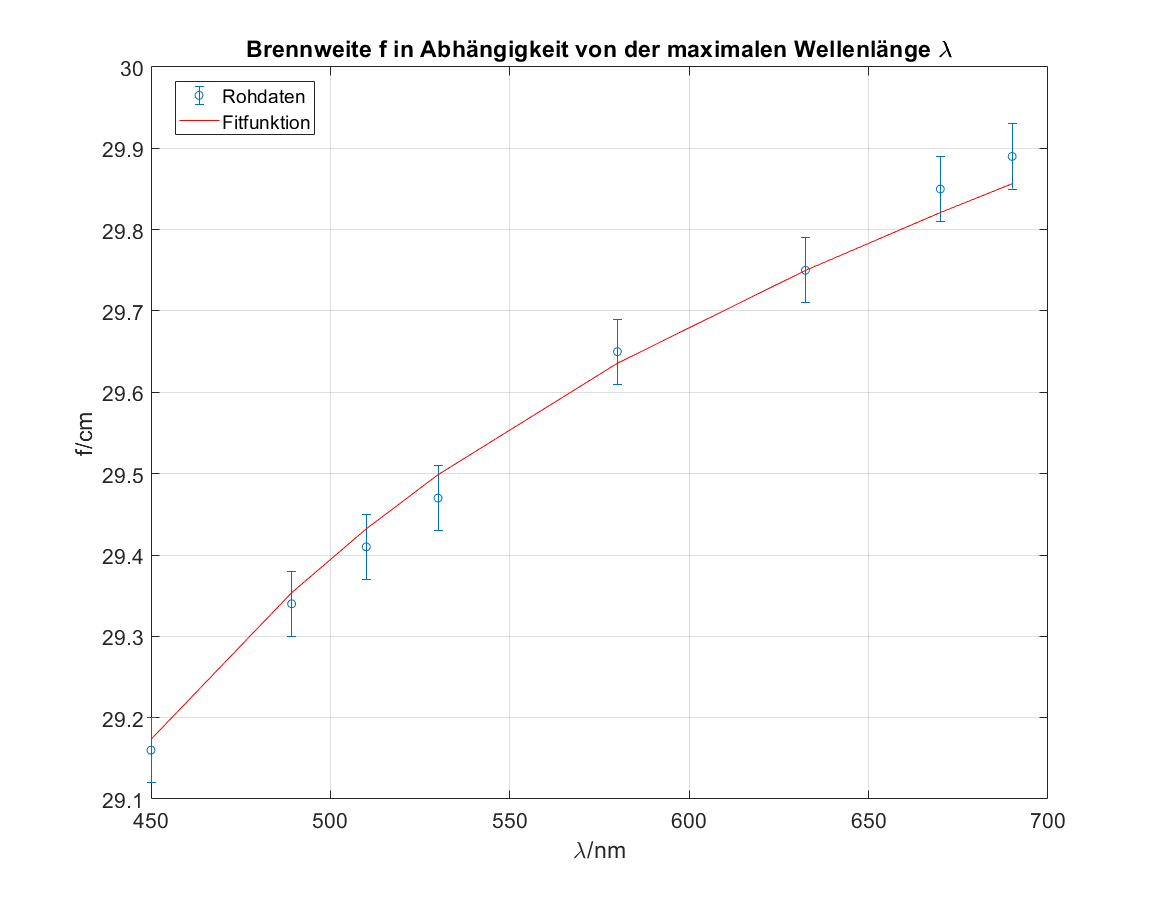
\includegraphics[width=0.7\textwidth]{2023-05-08 - V4 - Geometrische Optik, optische Abbildung und Aberrationen/images/versuch1/chrom.png}
    \caption{Messwerte inkl. Fehlerbalken und Fit durch die Werte}
    \label{chrom}
\end{figure}
\end{document}